\section{Proposal's context, positioning and objective(s)}
\label{sec:context}

\subsection{a. Objectives and scientific hypotheses}

\Comments{Present the objectives and the research hypotheses ; present the scientific and technical barriers to be lifted ; present the expected results; if applicable describe any final products developed.}

\subsection{b. Originality and relevance in relation to the state of the art}

\Comments{Emphasise the ambitious nature of the proposal and the novelty of the research in relation to the state of the art ; show the possible contributions of project partners to the state of the art ; present any preliminary results. In the case of a project proposal following up on previous project(s) already funded by ANR or by another body, provide a summary of the results achieved and clearly describe the new issues raised and the new objectives set out in the light of the earlier project.}

\subsection{c. Methodology and risk management}

\Comments{Describe the methods and technical decisions, risks and fall-back solutions envisaged.}

\subsection{pre-proposition}

%version 2, pour avoir une entree en mathiere plus grand public. 
\noindent\textbf{Context.} 
3D volumes come from the segmentation of magnetic resonance, X-ray tomographic or micro-tomographic images. 
They are also generated in scientific modelling and by voxel editors. 
This project is about the geometry of volume boundaries, called \emph{digital surfaces} (fig.~\ref{sub:snow}). 
Keeping the digital nature of the data is an advantage
to use efficient spatial data structures such as voxel octree, 
to perform constructive solid geometry operations,
to do integer-only and exact computations, etc.
A drawback is its poor geometry, because at any resolution a digital surface is only 
made up of quadrangular surface element (\emph{surfel} for short) 
whose normal vector is parallel to one axis. 
Many tasks in computer graphics, vision and 3D image analysis require a richer geometry: 
rendering, surface deformation for simulation or tracking, precise geometric measurements, etc.
To perform relevant geometric tasks and 
to benefit from the above-mentioned advantages in the same time, 
we need to enhance the geometry of digital surfaces by estimating extra data for each surfel. 
This project focuses on estimations of local and first-order geometric quantities: 
normal vector, distance to boundary, coverage of the inner and outer incident voxels 
(see fig.~\ref{sub:2D} for a 2D illustration).  


\begin{figure}[hb]
 \subfloat[]{ 
 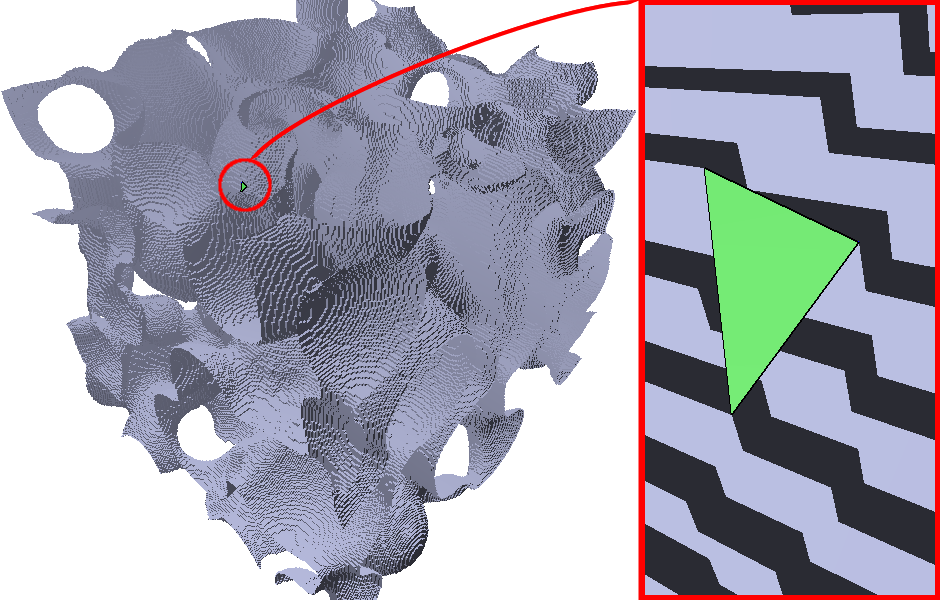
\includegraphics[height=0.2\textheight]{snow-compositionv2.png} %width=0.55\textwidth
 \label{sub:snow}
 }
% \subfloat[]{
%  \includegraphics[width=0.25\textwidth,angle=90,origin=b,trim=40 40 10 60,clip=true]{onPlane2-6-11.eps} %
% \label{sub:pattern}
% }
 \subfloat[]{
  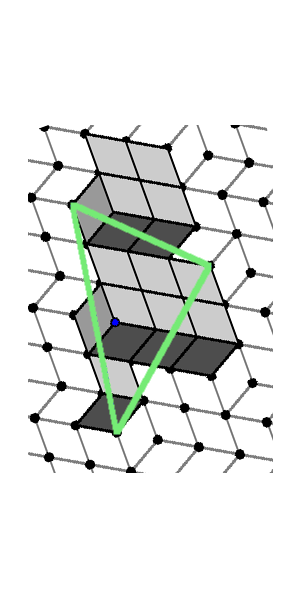
\includegraphics[height=0.2\textheight]{pattern-green.png} %
 \label{sub:pattern}
 }
 \subfloat[]{
\begin{tabular}[b]{cc}
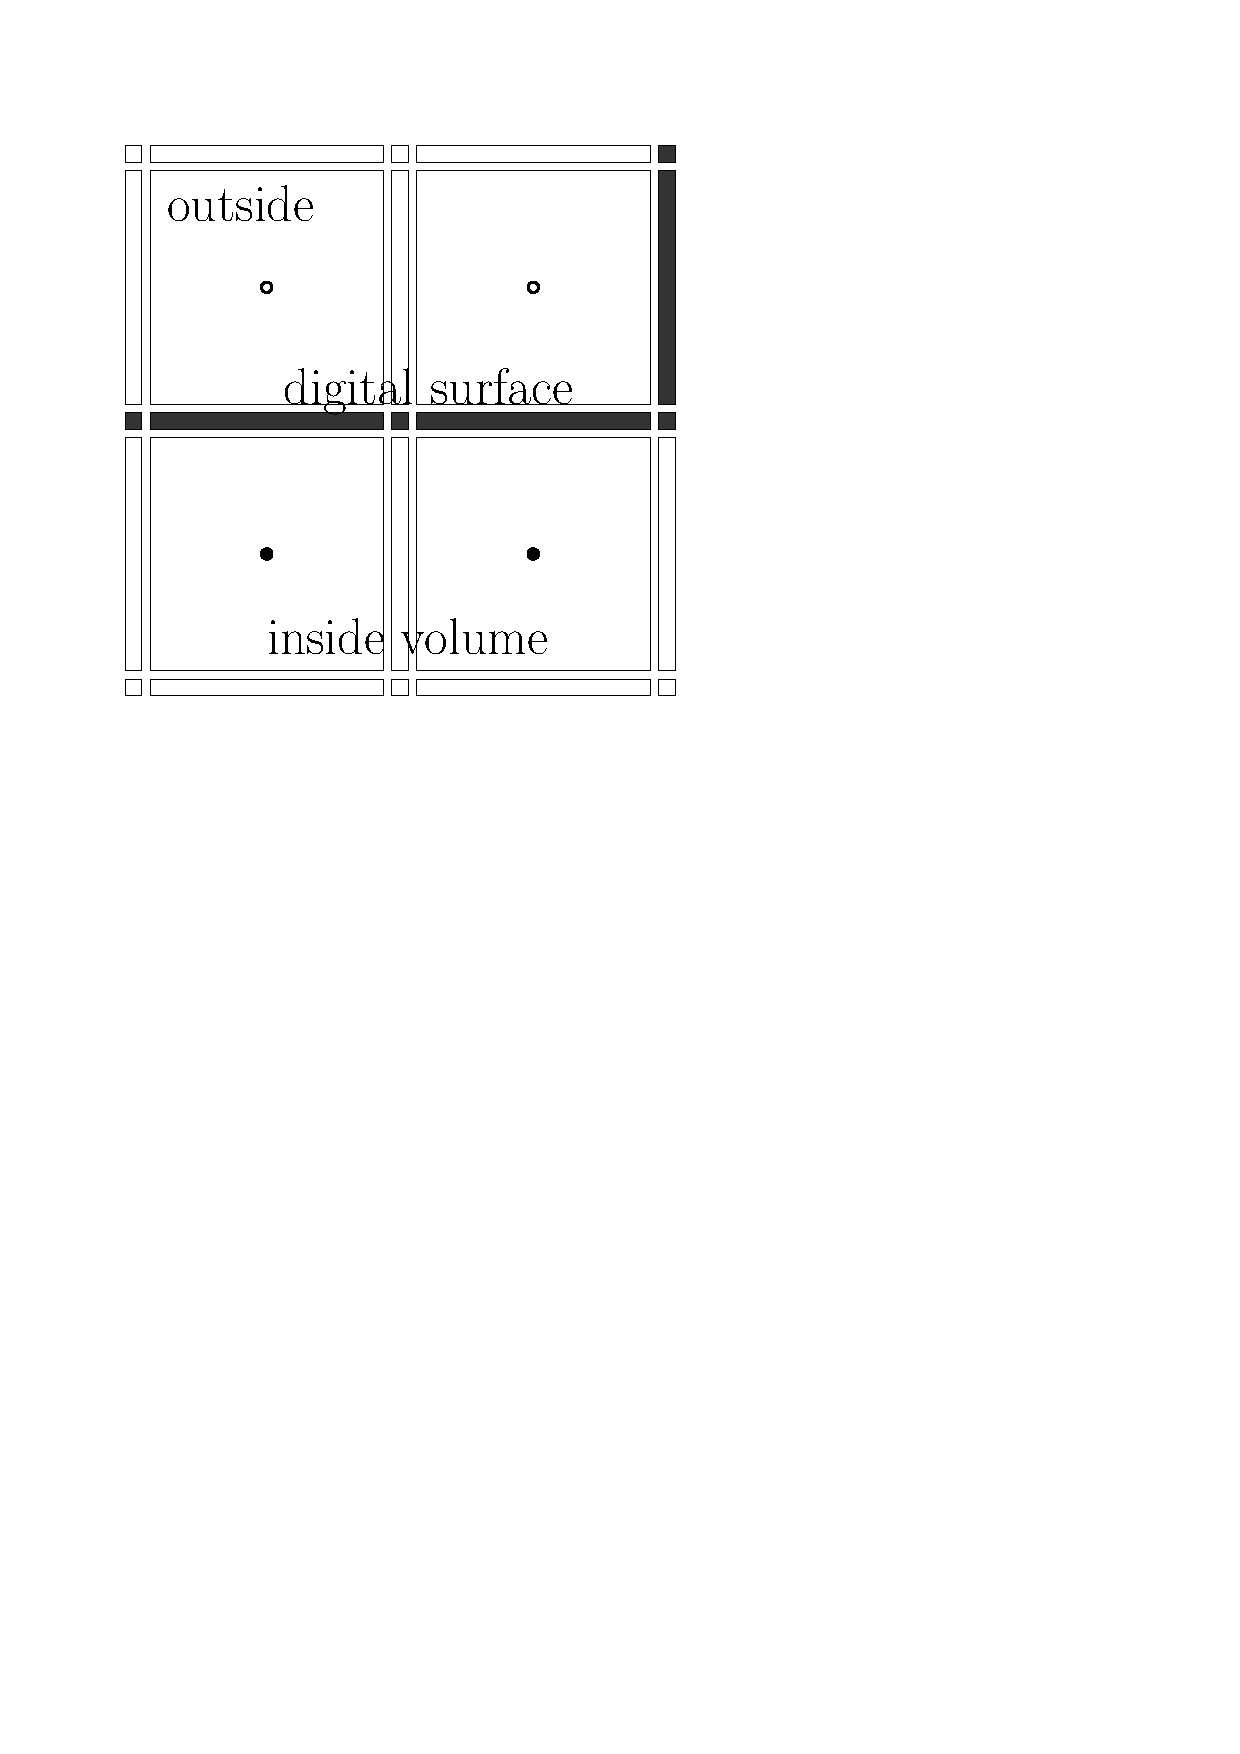
\includegraphics[width=0.145\textwidth,page=1]{square.pdf} &
\includegraphics[width=0.145\textwidth,page=2]{square.pdf} \\
\includegraphics[width=0.145\textwidth,page=3]{square.pdf} &
\includegraphics[width=0.145\textwidth,page=4]{square.pdf} \\
\end{tabular}
 \label{sub:2D}
 }
% \subfloat[]{ 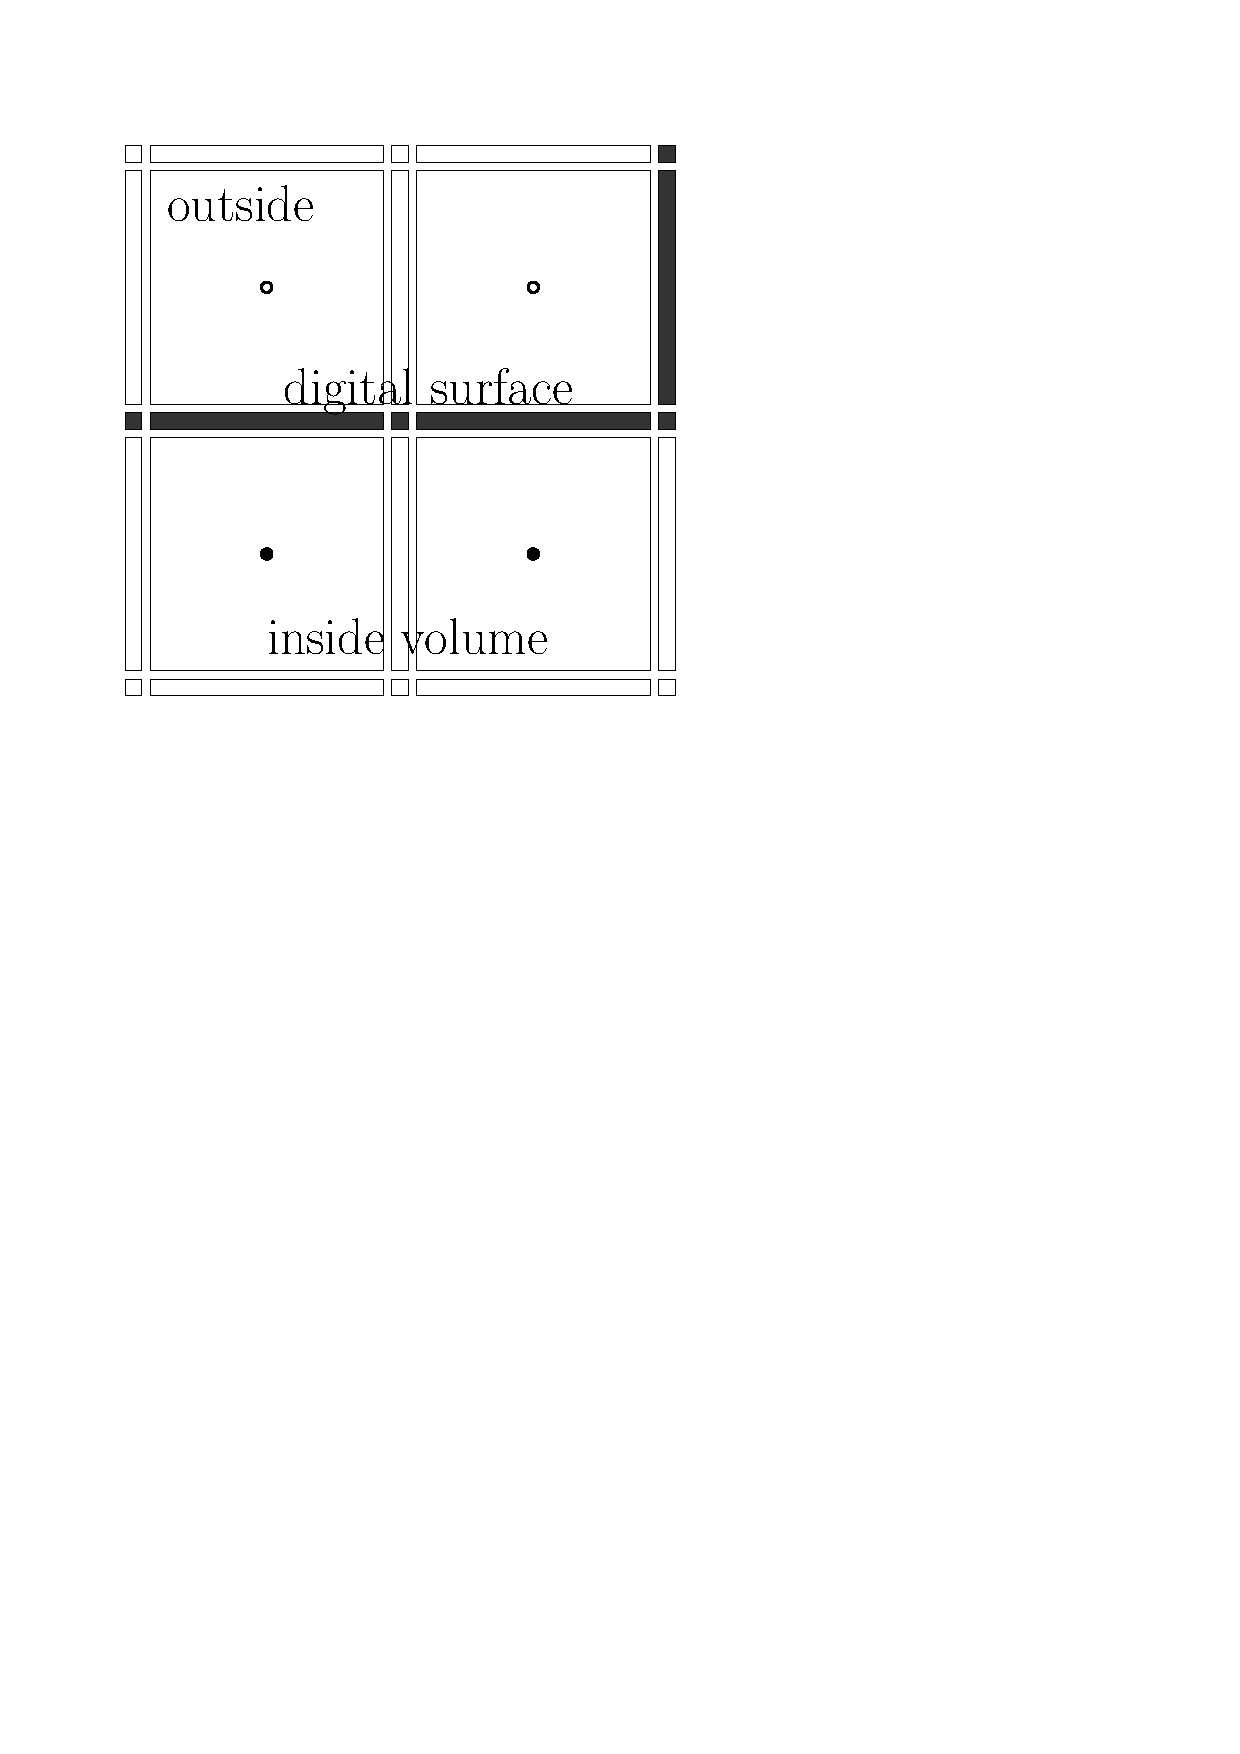
\includegraphics[width=0.17\textwidth,page=1]{square.pdf} } \hspace{0.05\textwidth}
% \subfloat[]{ \includegraphics[width=0.17\textwidth,page=2]{square.pdf} } \hspace{0.05\textwidth}
% \subfloat[]{ \includegraphics[width=0.17\textwidth,page=3]{square.pdf} } \hspace{0.05\textwidth}
% \subfloat[]{ \includegraphics[width=0.17\textwidth,page=4]{square.pdf} } 
 \caption{(a) ``ice-air'' interface in a micro-tomographic image of snow\protect\footnotemark~with a closer view to a local normal vector estimated by computing a relevant facet. (b) Piece of digital plane that locally fits to the surface. (c) 2D illustration of a digital surface: voxels are big squares whose center is depicted by a black (resp. white) disk if it lies inside (resp. outside) the volume; surfels are elongated dark rectangles. We want to estimate a relevant normal vector at a given surfel (top right), but also locally reconstruct a boundary perpendicular to this normal vector in order to derive distance and coverage estimations (bottom row).} 
\label{fig:ex} 
\end{figure}
 %\dav{(former ANR Project digitalSnow)}.
\footnotetext{obtained by the 3SR Lab and CEN/CNRM - GAME URA 1357/M\'{e}t\'{e}o-France - CNRS, 
shared during ANR-11-BS02-009 DigitalSnow project.}

\noindent\textbf{Positioning and scientific bottleneck.}
The surface geometry within a patch around each surfel should be gathered to provide such estimations -- e.g. by convolution \cite{Pottmann2009} or polynomial fitting \cite{Cazals2008}.
Almost all methods require at least one parameter that controls the size of the patch.  

To the best of our knowledge, on digital surfaces, only one parameter-free normal estimator has been proposed in nD (see \cite{Lachaud2003} and references therein for 3D). It is based on maximal digital straight segments on 2D slices. Maximal digital straight segments provide windows of adaptive size but the slicing truncates the geometric information and leads to an artificial spatial variability because two neighbor surfels only share one slice over two.     
%David: II ?
%Tris: pour l'estimation de normale, c'est un peu over-kill, mais c'est juste, plus généralement pour toute les méthodes qui ont un parametre de taille (même si la convergence n'est pas prouvée). En parler dans la proposition...

Is it possible to provide \emph{accurate} and \emph{parameter-free} estimators based on a surface patch with \emph{adaptive} size?
%Note that accuracy will be evaluated in a \emph{multigrid-convervence} framework as described in section \ref{sec:wp}, WP2. 
Since we are looking for first-order estimations, the patch will be typically a piece of digital plane that locally fits to the digital surface (fig.~\ref{sub:pattern}). A challenge is to cover the whole digital surface by maximal pieces of digital plane. 
What makes the problem hard is that there is a combinatorial explosion of maximal pieces of digital plane \cite{Sivignon2009} and that among them, not all are tangent to the digital surface in a point set framework.  
Related works usually make grow a point set by a breadth-first search according to some heuristics and decide whether the current set is a piece of digital plane or not \cite{Sivignon2004,Charrier2011}. The results are highly dependent on the chosen heuristics.   
%TODO citation de David sur la reconnaissance de plans discrets ?

\noindent\textbf{Objectives.}
An opportunity to make a breakthrough in this issue is the recent development by the principal investigator and its collaborators of \emph{plane-probing} algorithms \cite{LPRTCS2016, LPRDGCI2016, LPRJMIV2017}. These algorithms decide on-the-fly how to probe the digital surface and make grow a piece of digital plane, which is tangent by construction. The growth direction is given by both arithmetic and geometric properties.

The first goal of this project is to study extra arithmetic and combinatorial properties of plane-probing algorithms (see WP0 and WP1 in section~\ref{sec:wp}, describing work packages). The second one is to derive \emph{efficient}, \emph{accurate} and \emph{parameter-free} estimators of \emph{local} and \emph{first-order} geometric quantities (WP2). The third one is to provide a method and a tool for an automatic and \emph{multiscale} analysis of digital surfaces (WP3). 
Since there are so many perspectives and paths to follow, this project needs to strengthen a team of experts by full-time workers in order to make the best of them. 
%a person working full-time in a team of experts in order to make the best of them. 
